%  Template file for an a0 landscape poster.
% Written by Graeme, 2001-03 based on Norman's original microlensing
% poster.
%
% See discussion and documentation at
% <http://www.astro.gla.ac.uk/users/norman/docs/posters/>
%
% $Id: poster-template-landscape.tex,v 1.2 2002/12/03 11:25:46 norman Exp $


% Default mode is landscape, which is what we want, however dvips and
% a0poster do not quite do the right thing, so we end up with text in
% landscape style (wide and short) down a portrait page (narrow and
% long). Printing this onto the a0 printer chops the right hand edge.
% However, 'psnup' can save the day, reorienting the text so that the
% poster prints lengthways down an a0 portrait bounding box.
%
% 'psnup -w85cm -h119cm -f poster_from_dvips.ps poster_in_landscape.ps'

\documentclass[a0]{a0poster}
% You might find the 'draft' option to a0 poster useful if you have
% lots of graphics, because they can take some time to process and
% display. (\documentclass[a0,draft]{a0poster})
\input defs
\pagestyle{empty}
\setcounter{secnumdepth}{0}
\renewcommand{\familydefault}{\sfdefault}
\newcommand{\QED}{~~\rule[-1pt]{8pt}{8pt}}\def\qed{\QED}

\renewcommand{\reals}{{\mbox{\bf R}}}

% The textpos package is necessary to position textblocks at arbitary
% places on the page.
\usepackage[absolute]{textpos}

\usepackage{fleqn,psfrag,wrapfig,tikz}

\usepackage[papersize={38in,28in}]{geometry}

% Graphics to include graphics. Times is nice on posters, but you
% might want to switch it off and go for CMR fonts.
\usepackage{graphics}


% we are running pdflatex, so convert .eps files to .pdf
%\usepackage[pdftex]{graphicx}
%\usepackage{epstopdf}

% These colours are tried and tested for titles and headers. Don't
% over use color!
\usepackage{color}
\definecolor{Red}{rgb}{0.9,0.0,0.1}

\usepackage{amsmath}
\usepackage{amsfonts}
\usepackage{hyperref}
\usepackage{subfig}
\usepackage{verbatim}

\definecolor{bluegray}{rgb}{0.15,0.20,0.40}
\definecolor{bluegraylight}{rgb}{0.35,0.40,0.60}
\definecolor{gray}{rgb}{0.3,0.3,0.3}
\definecolor{lightgray}{rgb}{0.7,0.7,0.7}
\definecolor{darkblue}{rgb}{0.2,0.2,1.0}
\definecolor{darkgreen}{rgb}{0.0,0.5,0.3}

\renewcommand{\labelitemi}{\textcolor{bluegray}\textbullet}
\renewcommand{\labelitemii}{\textcolor{bluegray}{--}}

\setlength{\labelsep}{0.5em}


% see documentation for a0poster class for the size options here
\let\Textsize\normalsize
%\def\Head#1{\noindent\hbox to \hsize{\hfil{\LARGE\color{bluegray} #1}}\bigskip}
\def\Head#1{\noindent{\LARGE\color{bluegray} #1}\bigskip}
\def\LHead#1{\noindent{\LARGE\color{bluegray} #1}\bigskip}
\def\Subhead#1{\noindent{\large\color{bluegray} #1}\bigskip}
\def\Title#1{\noindent{\VeryHuge\color{Red} #1}}


% Set up the grid
%
% Note that [40mm,40mm] is the margin round the edge of the page --
% it is _not_ the grid size. That is always defined as
% PAGE_WIDTH/HGRID and PAGE_HEIGHT/VGRID. In this case we use
% 23 x 12. This gives us three columns of width 7 boxes, with a gap of
% width 1 in between them. 12 vertical boxes is a good number to work
% with.
%
% Note however that texblocks can be positioned fractionally as well,
% so really any convenient grid size can be used.
%
\TPGrid[40mm,40mm]{23}{12}      % 3 cols of width 7, plus 2 gaps width 1

\parindent=0pt
\parskip=0.2\baselineskip

\begin{document}

% Understanding textblocks is the key to being able to do a poster in
% LaTeX. In
%
%    \begin{textblock}{wid}(x,y)
%    ...
%    \end{textblock}
%
% the first argument gives the block width in units of the grid
% cells specified above in \TPGrid; the second gives the (x,y)
% position on the grid, with the y axis pointing down.

% You will have to do a lot of previewing to get everything in the
% right place.

% This gives good title positioning for a portrait poster.
% Watch out for hyphenation in titles - LaTeX will do it
% but it looks awful.
\begin{textblock}{23}(0,0)
\Title{Empirical Study of $\text{TD}_{\gamma}$ Reinforcement Learning
       algorithms}
\end{textblock}

\begin{textblock}{23}(0,0.6)
{
\LARGE
Kirill Bobyrev
}

{
\Large
\color{bluegray}
\emph{Optimization Class Project. MIPT}
}
\end{textblock}


% Uni logo in the top right corner. A&A in the bottom left. Gives a
% good visual balance, but you may want to change this depending upon
% the graphics that are in your poster.
%\begin{textblock}{2}(0,10)
%Your logo here
%%\includegraphics{/usr/local/share/images/AandA.epsf}
%\end{textblock}

%\begin{textblock}{2}(21.2,0)
%Another logo here
%%\resizebox{2\TPHorizModule}{!}{\includegraphics{/usr/local/share/images/GUVIu/GUVIu.eps}}
%\end{textblock}


\begin{textblock}{7.0}(0,1.5)

\medskip
\hrule\medskip
\Head{Reinforcement Learning at a glance}\\

Reinforcement Learning is an area of machine learning concerned with how
\textit{agents} should take \textit{actions} in an \textit{environment} so as
to maximize the \textit{cumulative reward}.

\begin{center}
  \begin{figure}
    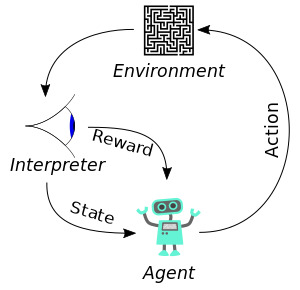
\includegraphics[width=0.45\textwidth]{figures/rl-intro-diagram.jpeg}
    \caption{Reinforcement Learning world model}
  \end{figure}
\end{center}

Reinforcement Learning problem is typically modelled by Markov Decision Process:

\begin{itemize}
  \item $\mathcal{S}$ --- set of states, it can be finitie or infinite, discrete
    or continuous
  \item $\mathcal{A}$ --- set of actions availible to the agent
  \item $P_a(s, s') = P(S_{t+1} = s' | S_t = s, A_t = a)$ --- probabilities of
    action $a$ in state $s$ leading to state $s'$
  \item $r_a(s, s') = r(S_{t+1} = s' | S_t = s, A_t = a)$ --- numerical reward
    distribution, a rule incorporated in the environment which indicates which
    reward is given to the agent upon taking action $a$ in state $s$ and
    resulting in state $s'$
  \item $\gamma \in [0, 1]$ --- discount factor which controls the relative
    difference in importance between the future and present rewards
\end{itemize}

It is often assumed that the transitional probabilities and reward distribution
are not directly availible to the agent. The goal of the Reinforcement Learning
agent is to maximize $\sum_{t=0}^{\infty} \gamma^t R_{a_{t}}(S_{t}, S_{t + 1})$
by finding the optimal policy $\pi: \mathcal{S} \times \mathcal{A} \rightarrow
[0, 1]$. In order to achieve this goal, the agent typically learns value
function $v_\pi(s) = \mathbb{E}[R] = {\mathbb{E}}[\sum_{t=0}^\infty \gamma^t R_t | S_0 = s]$

\begin{center}
\begin{figure}%
    \centering
    \subfloat[Atari 2600 games]{{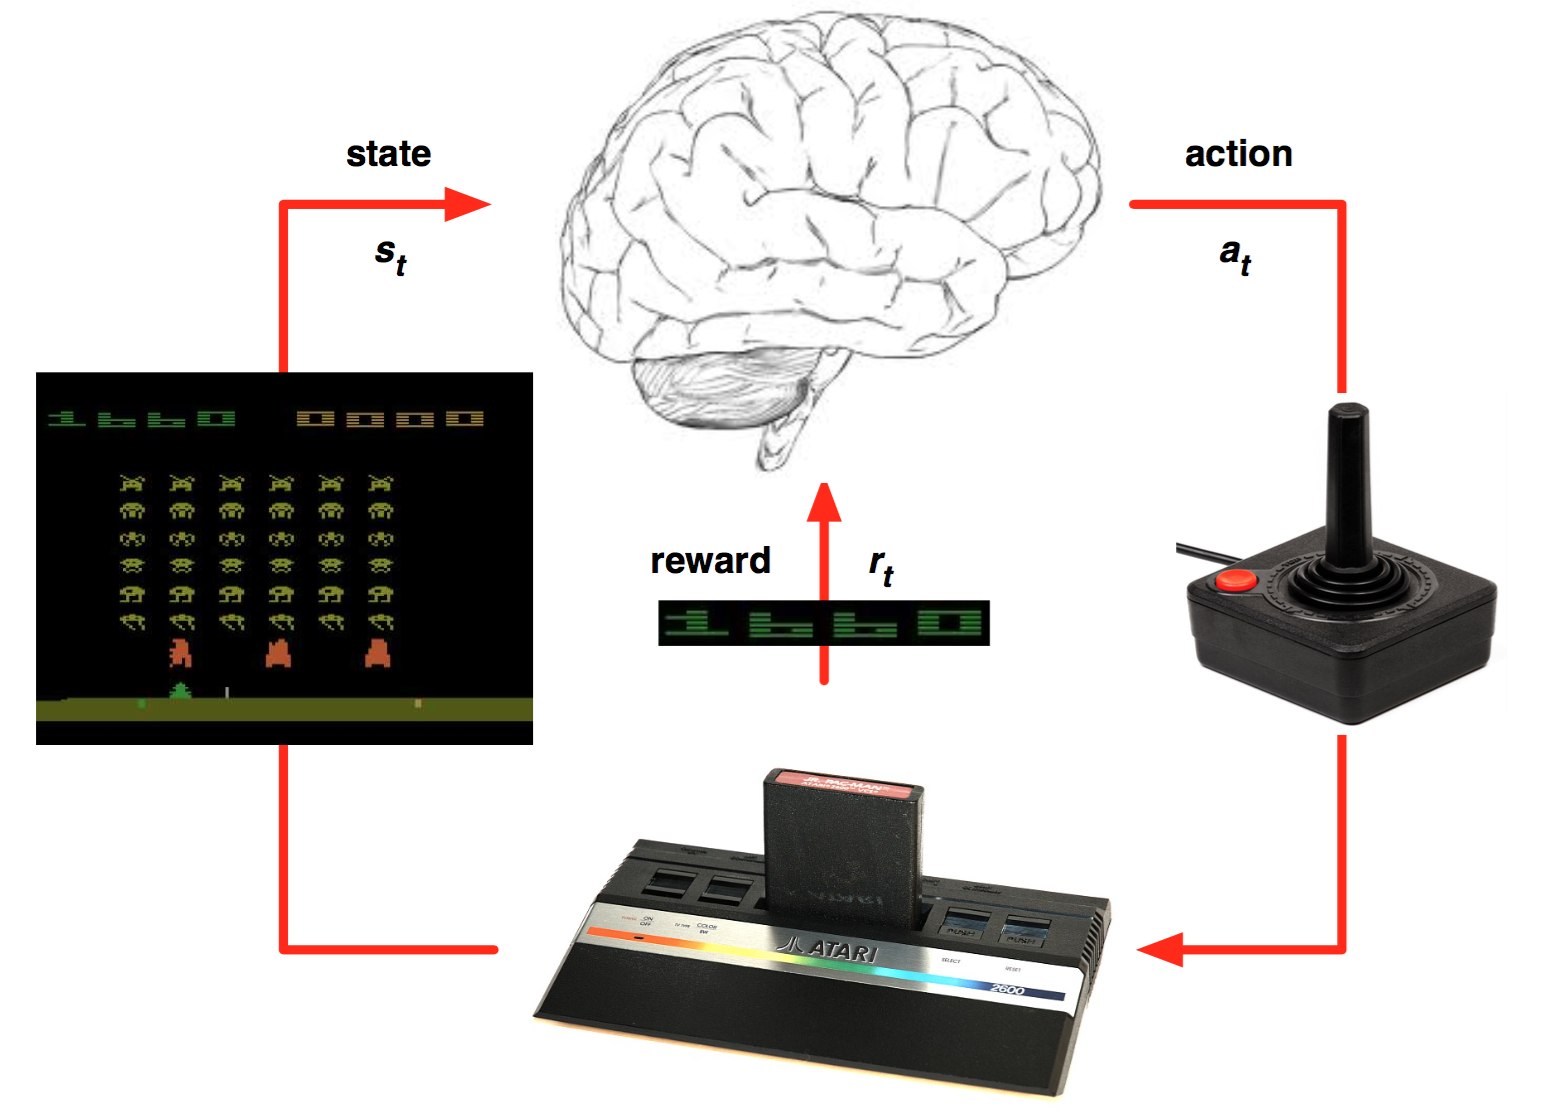
\includegraphics[width=0.40\textwidth]{figures/atari-environment-example.png}}}
    \qquad
    \subfloat[Sokoban]{{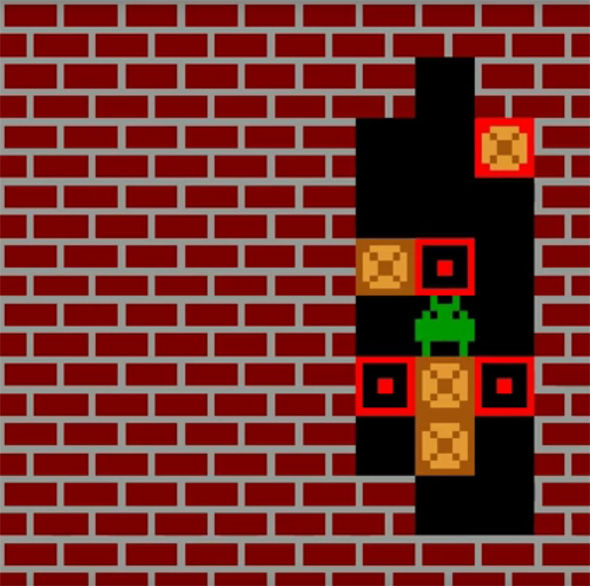
\includegraphics[width=0.40\textwidth]{figures/sokoban.jpg}}}
    \caption{Sample enfironments}%
    \label{fig:example}%
\end{figure}
\end{center}

\end{textblock}

\begin{textblock}{7.0}(8,1.5)

\medskip
\hrule\medskip
\Head{$\text{TD}(\gamma)$ Algorithm}\\

The main contribution of the studied paper is introducing the
$\text{TD}(\gamma)$ family of algorithms, which eliminates the $\lambda$
parameter. It is shown that $\text{TD}(\gamma)$ outperforms current
state-of-the-art algorithms, such as $\text{TD}(\lambda)$. The objective of any
value estimation algorithm is to minimize the following expression given a set
of trajectories sampled using a certain policy and a set of hyperparameters:
$E(\theta) = \frac{1}{2} \sum_{\tau \in T} \sum_{t = 0}^{l_\tau - 1}
{(R_{s_t^\tau}^\gamma - V_\theta(s_t^\tau))}^2$.

\noindent\rule[-5pt]{.9\textwidth}{0.4pt}
{\footnotesize
\begin{tabbing}
    {\bf Given:} A discount factor, $\gamma$ \\*[\smallskipamount]
    Let $\theta= \boldsymbol{0}$. \\
    {\bf for} each trajectory $\tau \in T$ {\bf do} \\
      \qquad \= Store $\phi_0$ in memory \\
      \> {\bf for} $u = 1$ to $l_\tau$ {\bf do} \\
      \> \qquad \= Store $\phi_u$ and $R_{u - 1}$ in memory \\
      \>  \> $\delta = \boldsymbol{0}$ \\
      \>  \> {\bf for} $t = 0$ to $u - 1$ {\bf do} \\
      \>  \> \qquad \= $\boldsymbol{a} = \phi_t - \gamma^{u - t} \phi_u$ \\
      \>  \>  \> $b = \sum_{i = t}^{u - 1} \gamma^{i - t} R_i$ \\
      \>  \>  \> $\boldsymbol{\delta} = \boldsymbol{\delta} + w(u - t, l_{\tau} - t)[\boldsymbol{\theta} \cdot \boldsymbol{a} - b] \phi_t$ \\
      \>  \> {\bf end for} \\
      \>  \> $\boldsymbol{\theta} = \boldsymbol{\theta} - \alpha \boldsymbol{\delta}$ \\
      \> {\bf end for} \\
      \> Discard all $\phi$ and $R$ from memory \\
    {\bf end for}
\end{tabbing}}
\noindent\rule[10pt]{.9\textwidth}{0.4pt}

\begin{center}
\begin{figure}
  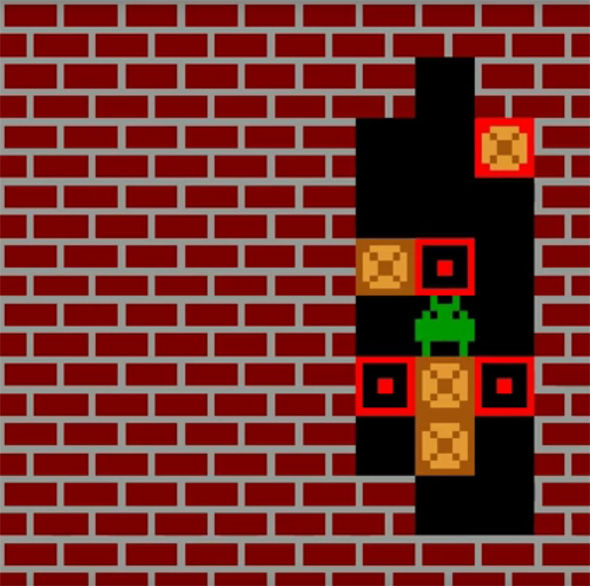
\includegraphics[width=0.35\textwidth]{figures/sokoban.jpg}
  \caption{\textbf{IMAGE IS PLACEHOLDER, ACTUAL SCHEME WILL BE ADDED SOON} Scheme of the implementation}%
\end{figure}
\end{center}

\medskip
\hrule\medskip
\Head{Importance of value estimation}\\

Even though the field has shifted towards \textit{Q-Learning} which
approximates $q_\pi(w, a) = \mathbb{E}[R] = \mathbb{E}[\sum_{t=0}^\infty R_t |
S_t = s, A_t = a]$, $\text{TD}(\gamma)$ can be used to improve the results of
state-of-the-art algorithms. By definition, $v_\pi(s) = \sum_{a \in
\mathcal{A}} q_\pi(s, a)$ and hence knowing the dynamics of the environment one
could efficiently navigate it using value function. However, in most cases the
transitional probabilities are not known to the agent. More sophisticated
methods like model-based Reinforcement Learning are able to deal with that
issue. Despite the additional complexity, such methods show good performance in
cases where thorough planning is crucial for the success of chosen approach. A
great example of such problem would be Sokoban where researchers used the
environment model to approximate model dynamics.

\end{textblock}

\begin{textblock}{7.0}(16,1.5)

\medskip
\hrule\medskip
\Head{Results}\\

Both $\text{TD}(\lambda)$ and $\text{TD}(\gamma)$ are benchmarked on rather
simple environment 19-Random-Walk. 19-Random-Walk consists of 19 non-terminal
states situated on a straight line and two terminal states at each end (one
with $-1$ and one with $+1$ reward, there availible actions are: move left and
move right. Such choice is satsified by the ability to solve Bellman equation
fairly easy and obtain true values for each state given a specific policy.

\begin{center}
\begin{figure}%
    \centering
    \subfloat[$\text{TD}({\lambda})$]{{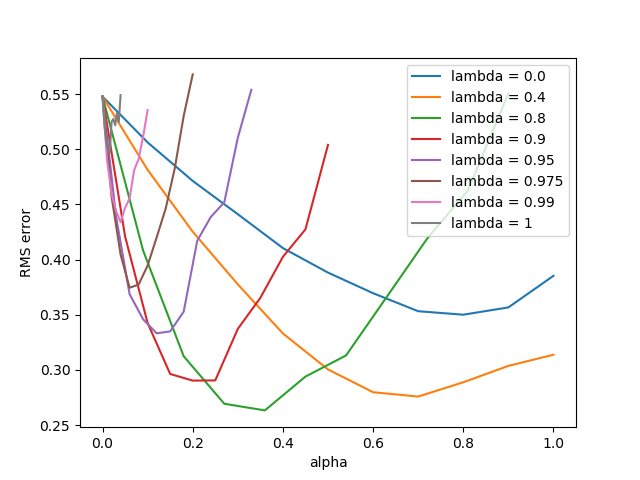
\includegraphics[width=0.46\textwidth]{figures/random-walk-td-lambda.png}}}
    \qquad
    \subfloat[$\text{TD}({\gamma})$]{{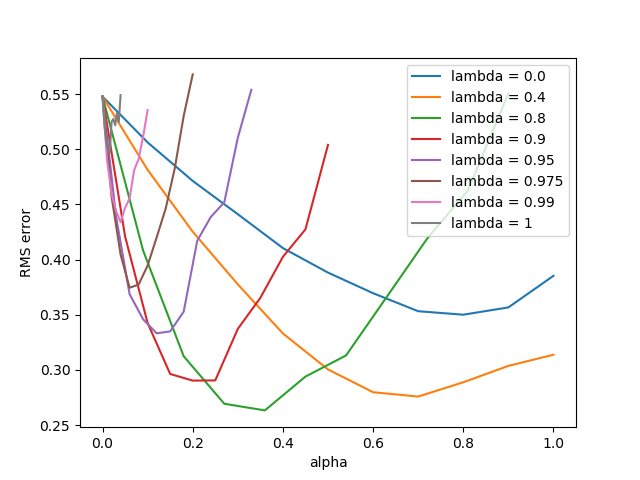
\includegraphics[width=0.46\textwidth]{figures/random-walk-td-lambda.png}}}
    \caption{Performance comparison}%
    \label{fig:results}%
\end{figure}
\end{center}

As shown on Figure~\ref{fig:results}, $\text{TD}(\gamma)$ shows superior
performance for the intermidiate settings of $\gamma$. However, the effect of
having lower variance of value estimate has its cost: while
$\text{TD}(\lambda)$ does not require the episode to terminate before operating
and even allows online setting, $\text{TD}(\gamma)$ does not have any of
mentioned advantages which makes it infeasible for continuous tasks.

\medskip
\hrule\medskip
\Head{Conclusion \& Future Work}\\

\medskip
\hrule\medskip
\Head{Additional materials \& Acknowledgements}\\

\LaTeX sources and supplementary materials can be found in the author's Github
repository:
\href{https://github.com/omtcvxyz/optimization-class-project}{omtcvxyz/optimization-class-project}.
Code for the experiments results reproduction is located in
\href{https://drive.google.com/file/d/1fmRALZn0-BRKlHWK\_juP9sswUdpEtCZ0/view?usp=sharing}{Google
Colab}. The experiments are based on Shangtong Zhang's work with further
intention to contribute the obtained results to main
\href{https://github.com/ShangtongZhang/reinforcement-learning-an-introduction}{reposotiry}
of Python implementation of ``Reinforcement Learning: An Introduction''.

\begin{comment}
\begin{thebibliography}{9}

\bibitem{TDGamma}
  George Konidaris, Scott Niekum, Philip S. Thomas,
  \href{https://papers.nips.cc/paper/4472-td_gamma-re-evaluating-complex-backups-in-temporal-difference-learning.pdf}{
  \textit{$\text{TD}_{\gamma}$: Re-evaluating Complex Backups in Temporal
          Difference Learning}},
  NIPS,
  2011.

\bibitem{Sutton}
  Richard Sutton and Andrew Barto,
  \href{http://incompleteideas.net/book/the-book-2nd.html}{\textit{Reinforcement Learning: An Introduction}},
  MIT Press, Cambridge, MA,
  Second edition,
  2018.

\bibitem{DQN}
  Volodymyr Mnih et al,
  \href{https://arxiv.org/abs/1312.5602}{\textit{Playing Atari with Deep Reinforcement Learning}},
  arXiv:1312.5602,
  2013.

\bibitem{Sokoban}
  Théophane Weber, Sébastien Racanière et al,
  \href{https://arxiv.org/abs/1707.06203}{\textit{Imagination-Augmented Agents for Deep Reinforcement Learning}},
  arXiv:1707.06203,
  2017.

\end{thebibliography}
\end{comment}.

\end{textblock}

\end{document}
